% Copyright 2004 by Till Tantau <tantau@users.sourceforge.net>.
%
% In principle, this file can be redistributed and/or modified under
% the terms of the GNU Public License, version 2.
%
% However, this file is supposed to be a template to be modified
% for your own needs. For this reason, if you use this file as a
% template and not specifically distribute it as part of a another
% package/program, I grant the extra permission to freely copy and
% modify this file as you see fit and even to delete this copyright
% notice. 

\documentclass{beamer}
\usepackage{subcaption}
% There are many different themes available for Beamer. A comprehensive
% list with examples is given here:
% http://deic.uab.es/~iblanes/beamer_gallery/index_by_theme.html
% You can uncomment the themes below if you would like to use a different
% one:
% \usetheme{AnnArbor}
% \usetheme{Antibes}
% \usetheme{Bergen}
% \usetheme{Berkeley}
% \usetheme{Berlin}
% \usetheme{Boadilla}
% \usetheme{boxes}
% \usetheme{CambridgeUS}
% \usetheme{Copenhagen}
% \usetheme{Darmstadt}
% \usetheme{default}
% \usetheme{Frankfurt}
% \usetheme{Goettingen}
% \usetheme{Hannover}
% \usetheme{Ilmenau}
% \usetheme{JuanLesPins}
% \usetheme{Luebeck}
\usetheme{Madrid}
% \usetheme{Malmoe}
% \usetheme{Marburg}
% \usetheme{Montpellier}
% \usetheme{PaloAlto}
% \usetheme{Pittsburgh}
% \usetheme{Rochester}
% \usetheme{Singapore}
% \usetheme{Szeged}
% \usetheme{Warsaw}

\title[COP 290]{Space Invaders}

% A subtitle is optional and this may be deleted
\subtitle{COP290: Assignment 3}

\author[Faran \and Kabir \and Kartikeya \and Prateek]{Faran Ahmad \and Kabir Chhabra \and Kartikeya Gupta \and Prateek Verma \\
  2013CS10220 \and 2013CS50287 \and 2013CS10231 \and 2013CS10246}
% - Give the names in the same order as the appear in the paper.
% - Use the \inst{?} command only if the authors have different
%   affiliation.

\institute[IITD] % (optional, but mostly needed)
{
  Department of Computer Science and Engineering\\
  IIT Delhi
}
% - Use the \inst command only if there are several affiliations.
% - Keep it simple, no one is interested in your street address.

\date{March 16, 2015}
% - Either use conference name or its abbreviation.
% - Not really informative to the audience, more for people (including
%   yourself) who are reading the slides online

\subject{Design Practices}
% This is only inserted into the PDF information catalog. Can be left
% out. 

% If you have a file called "university-logo-filename.xxx", where xxx
% is a graphic format that can be processed by latex or pdflatex,
% resp., then you can add a logo as follows:

% \pgfdeclareimage[height=0.5cm]{university-logo}{university-logo-filename}
% \logo{\pgfuseimage{university-logo}}

% Delete this, if you do not want the table of contents to pop up at
% the beginning of each subsection:
\AtBeginSubsection[]
{
  % \begin{frame}<beamer>{Outline}
  %   \tableofcontents[currentsection,currentsubsection]
  % \end{frame}
}

% Let's get started
\begin{document}

\begin{frame}
  \titlepage
\end{frame}

% \begin{frame}{Outline}
  % \tableofcontents
  % You might wish to add the option [pausesections]
% \end{frame}

% Section and subsections will appear in the presentation overview
% and table of contents.

\begin{frame}{Objectives}{}
  % \begin{itemize}
  % \item {
  %   My first point.
  % }
  % \item {
  %   My second point.
  % }
  % \end{itemize}
  Problem statement in brief
\end{frame}

\begin{frame}{Our choice}{Space Invaders}
    \begin{figure}[ht!]
      \centering
    %   \begin{subfigure}{.5\textwidth}
    %       \centering
          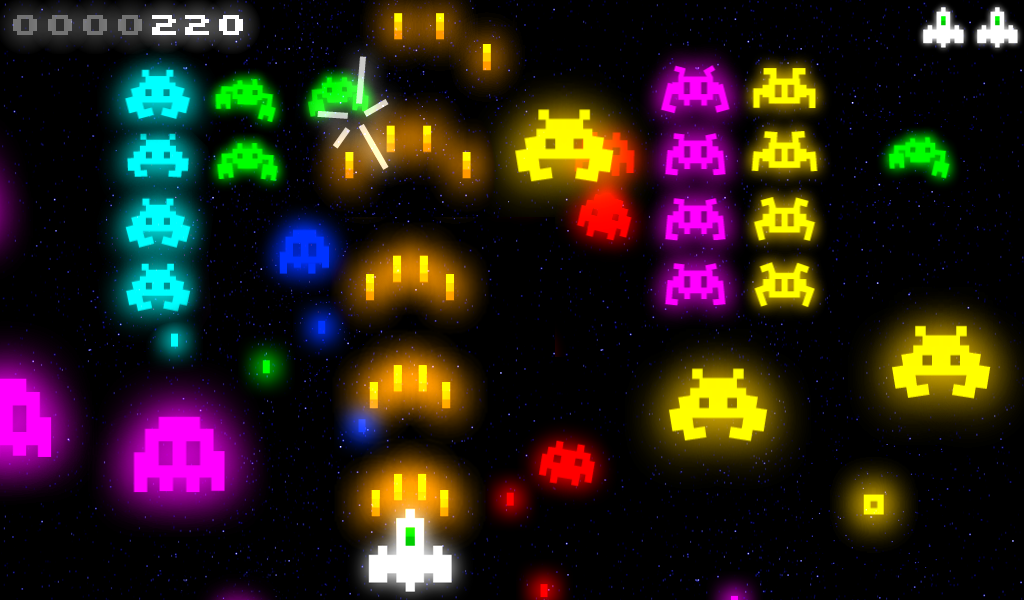
\includegraphics[width=1.0\linewidth]{gameplay.png}
    %       \caption{Sparse reconstruction}
    %       \label{fig:sub1}
    %   \end{subfigure}%
    %   \begin{subfigure}{.5\textwidth}
    %       \centering
    %       \includegraphics[width=1.0\linewidth]{dense_chariot.png}
    %       \caption{Dense reconstruction}
    %       \label{fig:sub2}
    %   \end{subfigure}
    %   % \caption{3D reconstruction}
    %   \label{figstart}
    \end{figure}
    % Image of the game
\end{frame}


\begin{frame}{Space Invaders}{Basic Game-play}
  \begin{itemize}
  	\item The player will control a space ship and shoot down aliens.
  	\item The aliens will shoot bullets at the players ship.
  	\item On getting hit by bullets the player will lose 1 life.
  	\item On destroying a large number of aliens, the player will get bonus lives.
  \end{itemize}
\end{frame}

\begin{frame}{Space Invaders}{Multi-player Version 1}
	\begin{itemize}
		\item In co-op mode, the different players will team up to fight the aliens.
		\item The points scored by each will be combined together.
	\end{itemize}
\end{frame}

\begin{frame}{Space Invaders}{Multi-player Version 2}
	About competitive mode
	\begin{itemize}
		\item In another mode, players will compete with each other.
		\item They will be put up against the same aliens but their scores will be separate. 
		\item The one who kills more aliens and / or survives the longest will get a higher score.
	\end{itemize}  
\end{frame}

\begin{frame}{Space Invaders}{Scoring Scheme - 1}
	\begin{block}{Lives}
		\begin{itemize}
			\item Each player will be given 3 lives.
			\item On getting hit by an alien bullet or colliding with an alien, a life will be lost.
			\item After killing 10 aliens in a row without any waste shot, a life will be awarded.
		\end{itemize}
	\end{block}
	
	\begin{block}{Scoring}
		\begin{itemize}
			\item On killing an alien a point would be avoided.
			\item On killing more and more aliens in a row, a multiplying factor associated with points would increase.
		\end{itemize}
	\end{block}
\end{frame}

% \begin{frame}{Space Invaders}{Scoring Scheme -2}
% 	Score in multi mode 1 \\
% 	Socer in multi mode 2
% \end{frame}

\begin{frame}{Network Design}{}
	TODO: SOCCER
  % \begin{figure}[ht!]
  %   \centering
  %   \includegraphics[width=\linewidth]{our_pipeline.png}
  %   % \caption{Accuracy of accelerometer data across different devices (scale cm)\label{fig1}}
  % \end{figure}
\end{frame}

\begin{frame}{Network Design}{Some more}
	TODO: SOCCER
\end{frame}

\begin{frame}{Network Design}{Network Outages}
	TODO: SOCCER \\
	Something about replacing player with AI player of same level till network is back
    % \begin{figure}[ht!]
    %   \centering
    %   \begin{subfigure}{.5\textwidth}
    %       \centering
    %       \includegraphics[width=1.0\linewidth]{graph.jpg}
    %       \caption{Accuracy of accelerometer data across different devices (scale cm)}
    %       % \label{fig:sub1}
    %   \end{subfigure}%
    %   \begin{subfigure}{.5\textwidth}
    %       \centering
    %       \includegraphics[width=1.0\linewidth]{integration.jpg}
    %       \caption{Obtaining velocity and displacement from static accelerometer data}
    %       % \label{fig:sub2}
    %   \end{subfigure}
    %   % \caption{3D reconstruction}
    %   % \label{figstart}
    % \end{figure}

\end{frame}

\begin{frame}{Artificial Intelligence}{Enemy side}
	TODO: KC \\
	Write about it dodging bullets and shooting in the direction of the players
  % \begin{figure}[ht!]
  %   \centering
  %   \includegraphics[width=\linewidth]{Corrected.jpeg}
  %   \caption{Applying smoothening techniques}
  % \end{figure}
\end{frame}

\begin{frame}{Artificial Intelligence}{Player side}
	TODO: KC \\
	Write about it dodging bullets and shooting in the direction of the enemy and also about the accuracy it will have. Something like a player quality.
  % \begin{figure}[ht!]
  %   \centering
  %   \includegraphics[width=\linewidth]{Corrected.jpeg}
  %   \caption{Applying smoothening techniques}
  % \end{figure}
\end{frame}


\begin{frame}{Time Line}{}
	  
\end{frame}

\begin{frame}
\vfill
\begin{center}
\huge{Thank You}
\end{center}
\vfill
\end{frame}


\end{document}


